\documentclass[10pt]{exam}
\usepackage[phy]{template-for-exam}
\usepackage{tikz,tikzpingus,graphicx}
%\pinguloadlibrary{horse}
\usetikzlibrary{shadings,decorations.pathmorphing,arrows.meta,patterns}

\def\headsize{0.4}
      \def\elevatorwidth{2.5}
  
      \tikzstyle{person}=[ultra thick, orange!50, scale=0.8]
  
      \tikzset{
        elevator/.pic = {
          \begin{scope}[scale=0.8]
            \draw[fill=gray!30] 
              (-.2,-.05) rectangle (\elevatorwidth+.2,3.55);
            \draw[fill=white] 
              (0,0) rectangle (\elevatorwidth,3.5);
    
            %guide-line (for development)
            %\draw (\elevatorwidth/2,0) -- ++(0,4);
    
    
            \path (\elevatorwidth/2,3.9) coordinate (pulley);
            \draw (pulley) -- ++(0,-0.4);
            \filldraw[fill=gray] (pulley) circle (0.3);
            \filldraw[fill=gray!50] (pulley) circle (0.2);
            \draw[thick] (pulley) 
              ++(-0.3,1) --
              ++(0,-1)
              arc[start angle=-180, end angle=0, radius=0.3] --
              ++(0,1);
          \end{scope}
        }
      }


\newcommand{\printeqs}{
  \begin{center}
    \begin{tabular}{|*9c|}
      \hline 
      &&&&&&&&\\
      &
      $F_{NET}=ma$ &&
      $F_{NET}=\pm F_1 \pm F_2 \pm \cdots$ &&
      $F_G=mg$ &&
      $g=\SI{9.8}{\meter\per\second^2}$ &
      \\
      \hline
    \end{tabular}
  \end{center}
}
\title{Newton's Law Concept Questions}
\author{Rohrbach}
\date{\today}

\begin{document}
\maketitle


\section*{Constancy of Free Fall}

In the famous Leaning Tower of Pisa experiment, Galileo dropped two balls from the top of the tower.  Let's say that one was 5~kg and the other was 500~kg
\vspace{1em}

  \begin{parts}
    \part Calculate the weight of the 5-kg ball. \vs
    \part Calculate the weight of the 500-kg ball. \vs
    \part Newton's Second Law says that the ball with more force (\emph{i.e.} more weight) should have a greater acceleration.  How can both balls have the same acceleration?
  \end{parts}

  \begin{tikzpicture}
    \node[anchor=north east] at (0,0) {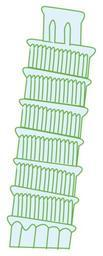
\includegraphics[scale=0.3]{pisa.jpg}};
    \draw[fill=gray] (0.2,-0.5) circle (0.1);
    \draw[fill=gray] (1,-0.5) circle (0.3);

  \end{tikzpicture}


\section*{Horse and Cart}

Calculate the net force in each of the free-body diagrams that have equal and opposite forces:

\tikzset{f/.append style={-{Stealth[length=3mm,width=2mm]}}}

\newcommand{\hforce}[2]
{
  \draw[f] (a) -- ++(#1, 0) 
        node[anchor=south] {#2};
}
\newcommand{\vforce}[2]
{
  \draw[f] (a) -- ++(0, #1) 
        node[anchor=west] {#2};
}
  \begin{center}
    \begin{tikzpicture}[scale=0.5]
        \newcommand{\createFBD}[1]
          {
            \filldraw (a) circle [radius=0.15];
            \path (a) node {} 
              + (-3,2.5) node {} ;
          }

        \begin{scope}
          \node (a) at (-5,4) {};
          \createFBD{(a)}
          \vforce{ 2}{\SI{18}{\newton}}
          \vforce{-2}{\SI{18}{\newton}}

        \end{scope}

        \begin{scope}
          \node (a) at (4,4) {};
          \createFBD{(c)}
          \vforce{ 2}{\SI{5}{\newton}}
          \vforce{-2}{\SI{5}{\newton}}
          \hforce{ 3}{\SI{7}{\newton}}
          \hforce{-3}{\SI{7}{\newton}}
        \end{scope}

      \end{tikzpicture}
    \end{center}

\noindent
A horse pulls a cart with a force of 400 Newtons forward.  However, according to Newton's Third Law, whenever the horse pulls the cart, there is an equal and opposite reaction of the cart pulling the horse of 400 N backwards.  Why do these two forces not cancel each other out giving to a net force of zero?

\tikzstyle{wheel}=[line width=10pt, fill=white]

  \vs
  \begin{center}
      \begin{tikzpicture}[scale=0.4]
        \pingu[on horse,body=white, body front=white,small size, left eye color=white, right eye color=white,feet color=brown,bill color=white]
        \draw[rounded corners, fill=gray] 
          (0,-2) rectangle ++(7,-0.5);
        \draw[rounded corners, fill=gray] 
          (6,-1) -- ++(7,0) -- ++(-1,-4) -- ++(-5,0) -- cycle;
        \draw[wheel] (7,-5) circle (1);
        \draw[wheel] (12,-5) circle (1);
        \fill[pattern=north east lines] (-6,-6.3) rectangle ++(21, -0.5);
      \end{tikzpicture}
  \end{center}
  \vs

  \pagebreak



\section*{Elevator Effect}
When do you are riding in an elevator, there are some times that you feel heavier and some times that you feel lighter.

\vspace{1em}


  \def\headsize{0.4}
  \def\elevatorwidth{2.5}

  \tikzstyle{person}=[ultra thick, orange!50, scale=0.8]

  \tikzset{
    elevator/.pic = {
      \draw[fill=gray!30] 
        (-.2,-.05) rectangle (\elevatorwidth+.2,4.05);
      \draw[fill=white] 
        (0,0) rectangle (\elevatorwidth,4);

      %guide-line (for development)
      %\draw (\elevatorwidth/2,0) -- ++(0,4);


      \path (\elevatorwidth/2,4.4) coordinate (pulley);
      \draw (pulley) -- ++(0,-0.4);
      \filldraw[fill=gray] (pulley) circle (0.3);
      \filldraw[fill=gray!50] (pulley) circle (0.2);
      \draw[thick] (pulley) 
        ++(-0.3,1) --
        ++(0,-1)
        arc[start angle=-180, end angle=0, radius=0.3] --
        ++(0,1);
    }
  }


  \begin{center}
    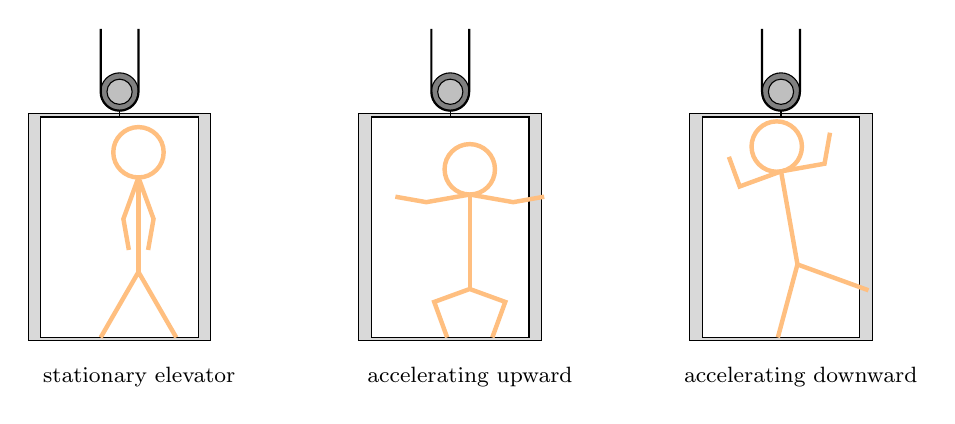
\begin{tikzpicture}

      \begin{scope}
        \path (0,0) pic{elevator} coordinate (start);

        \begin{scope}[person]
          \draw (start) 
          ++(.95,0) coordinate (left foot) --
          ++(60:1.2) coordinate (waist) --
          ++(-60:1.2) coordinate (right foot);

          \draw (waist)
            -- ++(90:1.5) coordinate (neck);
          \draw (neck) 
            ++(90:\headsize) circle (\headsize);
          \draw (neck)
            -- ++(-70:0.7) coordinate (right elbow)
            -- ++(-100:0.5) coordinate (right hand);
          \draw (neck)
            -- ++(-110:0.7) coordinate (left elbow)
            -- ++(-80:0.5) coordinate (left hand);
        \end{scope}

        \draw (start) ++(\elevatorwidth/2,-0.5)
          node {\footnotesize stationary elevator};

      \end{scope}

      \begin{scope}
        \path (4.2,0) pic{elevator} coordinate (start);


        \begin{scope}[person]
          \draw (start) 
          ++(1.2,0) coordinate (left foot) --
          ++(110:0.6) --
          ++(20:0.6) coordinate (waist) --
          ++(-20:0.6) --
          ++(250:0.6) coordinate (right foot);


          \draw (waist)
            -- ++(90:1.5) coordinate (neck);
          \draw (neck) 
            ++(90:\headsize) circle (\headsize);
          \draw (neck)
            -- ++(-10:0.7) coordinate (right elbow)
            -- ++(10:0.5) coordinate (right hand);
          \draw (neck)
            -- ++(190:0.7) coordinate (left elbow)
            -- ++(170:0.5) coordinate (left hand);
        \end{scope}

        \draw (start) ++(\elevatorwidth/2,-0.5)
          node {\footnotesize accelerating upward};

      \end{scope}

      \begin{scope}
        \path (8.4,0) pic{elevator} coordinate (start);

        \begin{scope}[person]
          \draw (start) 
          ++(1.2,0) coordinate (left foot) --
          ++(75:1.2) coordinate (waist) --
          ++(-20:1.2) coordinate (right foot);

          \draw (waist)
            -- ++(100:1.5) coordinate (neck);
          \draw (neck) 
            ++(100:\headsize) circle (\headsize);
          \draw (neck)
            -- ++(10:0.7) coordinate (right elbow)
            -- ++(80:0.5) coordinate (right hand);
          \draw (neck)
            -- ++(-160:0.7) coordinate (left elbow)
            -- ++(110:0.5) coordinate (left hand);
        \end{scope}

        \draw (start) ++(\elevatorwidth/2,-0.5)
          node {\footnotesize accelerating downward};

      \end{scope}

    \end{tikzpicture}
  \end{center}

  \vs[3]

  Which force corresponds to ``how heavy'' you feel?
  \vs

  How could you use an elevator to simulate weightlessness?
  \vs

  \paragraph{Example Problem} Let's say that a 75-kg person is standing in an elevator that is acceleration downward at 2.1~m/s$^2$.  What is the normal force acting on this person?  Do they feel heavier or lighter than usual?
  \vs[4]

\end{document}